\documentclass[11pt,a4paper]{article}

\usepackage{tadoc}

%\usepackage{amsmath,amssymb,amsfonts}
\usepackage{xcolor}
%\usepackage{graphicx}

\usepackage{minted}
\usemintedstyle{autumn}
\setminted{linenos,breaklines,tabsize=4,xleftmargin=1.5em}
%\usepackage{framed}

%\renewcommand{\multirowsetup}{\centering} 

\usepackage{pdfpages}


\title{VE572 --- Methods and Tools for Big Data}
\subtitle{Lab 1}
\author{\href{mailto:liuyh615@sjtu.edu.cn}{Yihao Liu}}
\semester{Summer}
\year{2019}
\blockinfo{
	\begin{center}
		\textbf{Goals of the lab}
	\end{center}	
	\begin{itemize}\itemsep .25cm
		\item Basic file input / output in Java
		\item Object-oriented programming in Java
	\end{itemize}	 
}

% whether or not to display the instructor line
\noinstructor

%\pagenumbering{gobble}

\begin{document}

\maketitle

\section{Introduction}

This lab requires you a strong background of C++ programming and helps you to turn it into the ability of Java programming. A simple guide can be found in the appendix \hyperlink{cpp2java}{cpp2java}.

...




\section{Appendix}
\hypertarget{cpp2java}{\ }
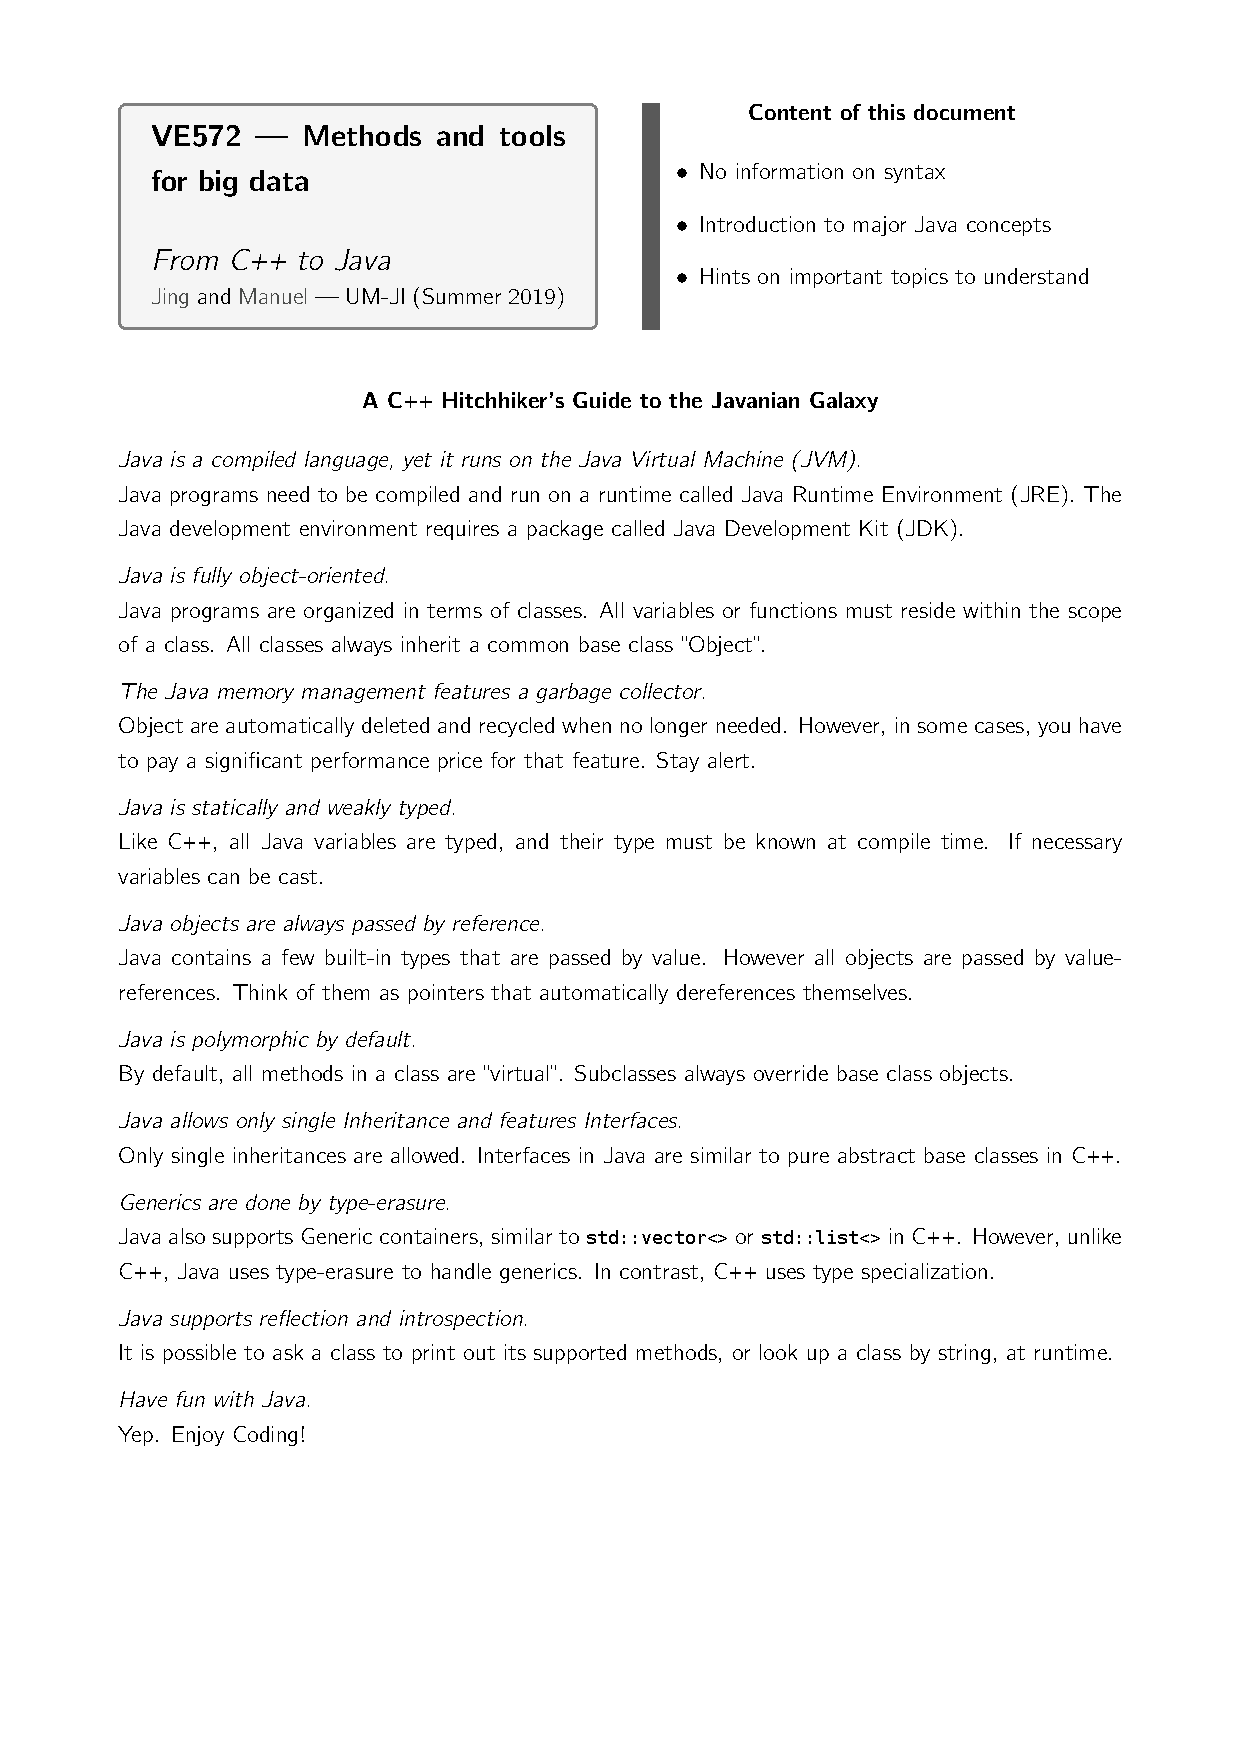
\includepdf{cpp2java.pdf}

\end{document}
